
\newpage

\section{Reti wireless}
Il wireless o senza fili indica una comunicazione tra dispositivi elettronici che non fa uso di cavi.

Generalmente il wireless utilizza onde radio a bassa potenza; tuttavia la definizione si estende anche ai dispositivi, meno diffusi, che sfruttano la radiazione infrarossa o il laser.

Ogni sistema di comunicazione wireless è composto da un trasmettitore, un ricevitore e dagli elementi deputati alla radiazione elettromagnetica ovvero alla trasduzione elettro-elettromagnetica e viceversa ovvero le antenne, i laser, i fotorivelatori.


\subsection{Wireless LAN - WLAN}
WLAN o wireless LAN è una rete locale (LAN) che sfrutta la tecnologia wireless, invece di una connessione cablata. In altre parole: con la sigla WLAN si indicano genericamente tutte le reti locali di computer che non utilizzano dei collegamenti via cavo per connettere fra loro gli host della rete; è una tecnologia definita da IEEE 802.11


\begin{multicols}{2}
    \begin{itemize}
        \item Pregi delle WLAN:
        \begin{itemize}
            \item Facilità di installazione
            \item Basso costo
            \item Assenza di cablaggio
            \item Mobilità
        \end{itemize}
    \end{itemize}
    \columnbreak
    \begin{itemize}
        \item Difetti delle WLAN:
        \begin{itemize}
            \item Inaffidabilità mezzo trasmissivo
            \item Sensibilità alle interferenze
            \item Privacy
        \end{itemize}
    \end{itemize}
\end{multicols}

\subsubsection{Infrastruttura WLAN}

"Il sistema è composto da un insieme di BSS interconnessi con un
Distribution System (DS) che collega i diversi Access Point (AP)"


\begin{figure}[h!]
    \centering
    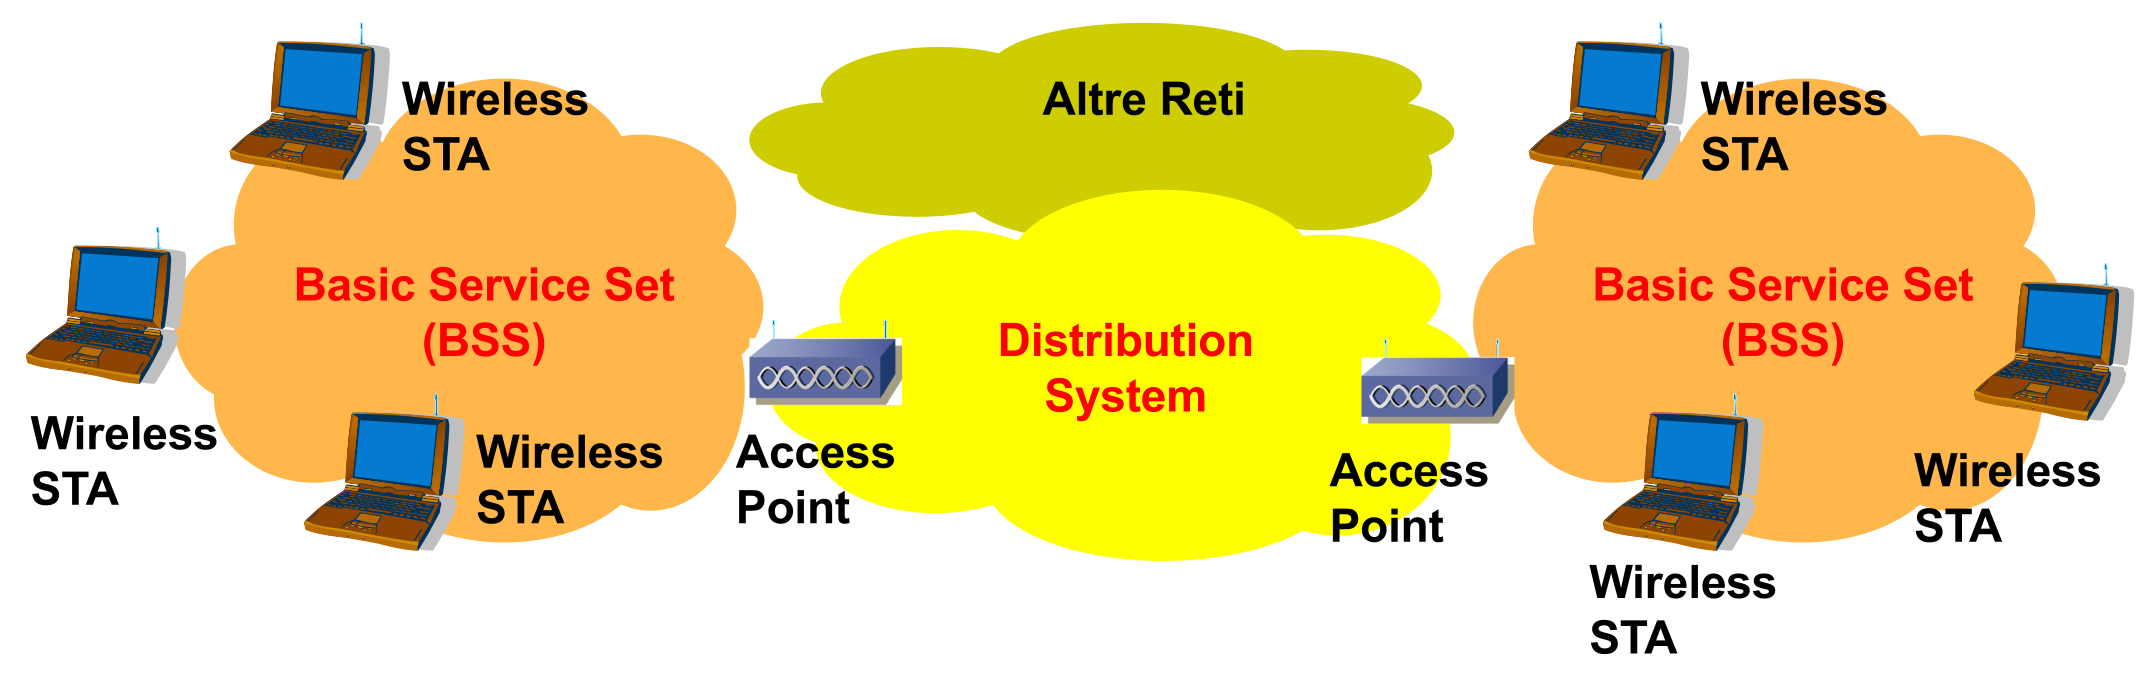
\includegraphics[scale=0.2]{images/infrastrutturawlan.png}
    \caption{Infrastruttura WLAN}
    \label{fig:infrastrutturawlan}
\end{figure}
Nelle aree arancioni, dette Basic service set (BSS), le wireless station comunicano nello stesso canale radio; ciò che permette la comunicazione tra questa area con altre sono gli access point (AP). 

\paragraph{Access point} tramite il dispositivo access point è possibile che le tecnologie ethernet 802.3 e le tecnologie wireless 802.11 possano scambiarsi informazioni, fungendo da ponte tra rete cablata e rete wireless.

Funge tra ponte anche tra reti wireless con canali radio differenti, poiché il dato passa da un access point all'altro, utilizzando ethernet.

\newpage

\paragraph{Famiglia 802.11x}

\begin{figure}[htbp]
    \centering
    \begin{minipage}{0.45\textwidth}
        La famiglia 802.11x è uno standard IEEE che definisce le caratteristiche di una WLAN.

        Lo standard 802.11x definisce una serie di tecniche di modulazione radio per segnali half-duplex che utilizzano di base lo stesso formato di dati. In particolare, la trasmissione si basa sul controllo di collisioni CSMA/CA per cui una emittente su uno specifico canale è in grado di determinare se su quello stesso canale ci siano altre entità che stanno trasmettendo (anche su protocolli diversi da quelli definiti da 802.11x) e trasmette le sue trame dati solo se il canale in quel momento è libero.
    \end{minipage}
        \hfill
    \begin{minipage}{0.53\textwidth}
        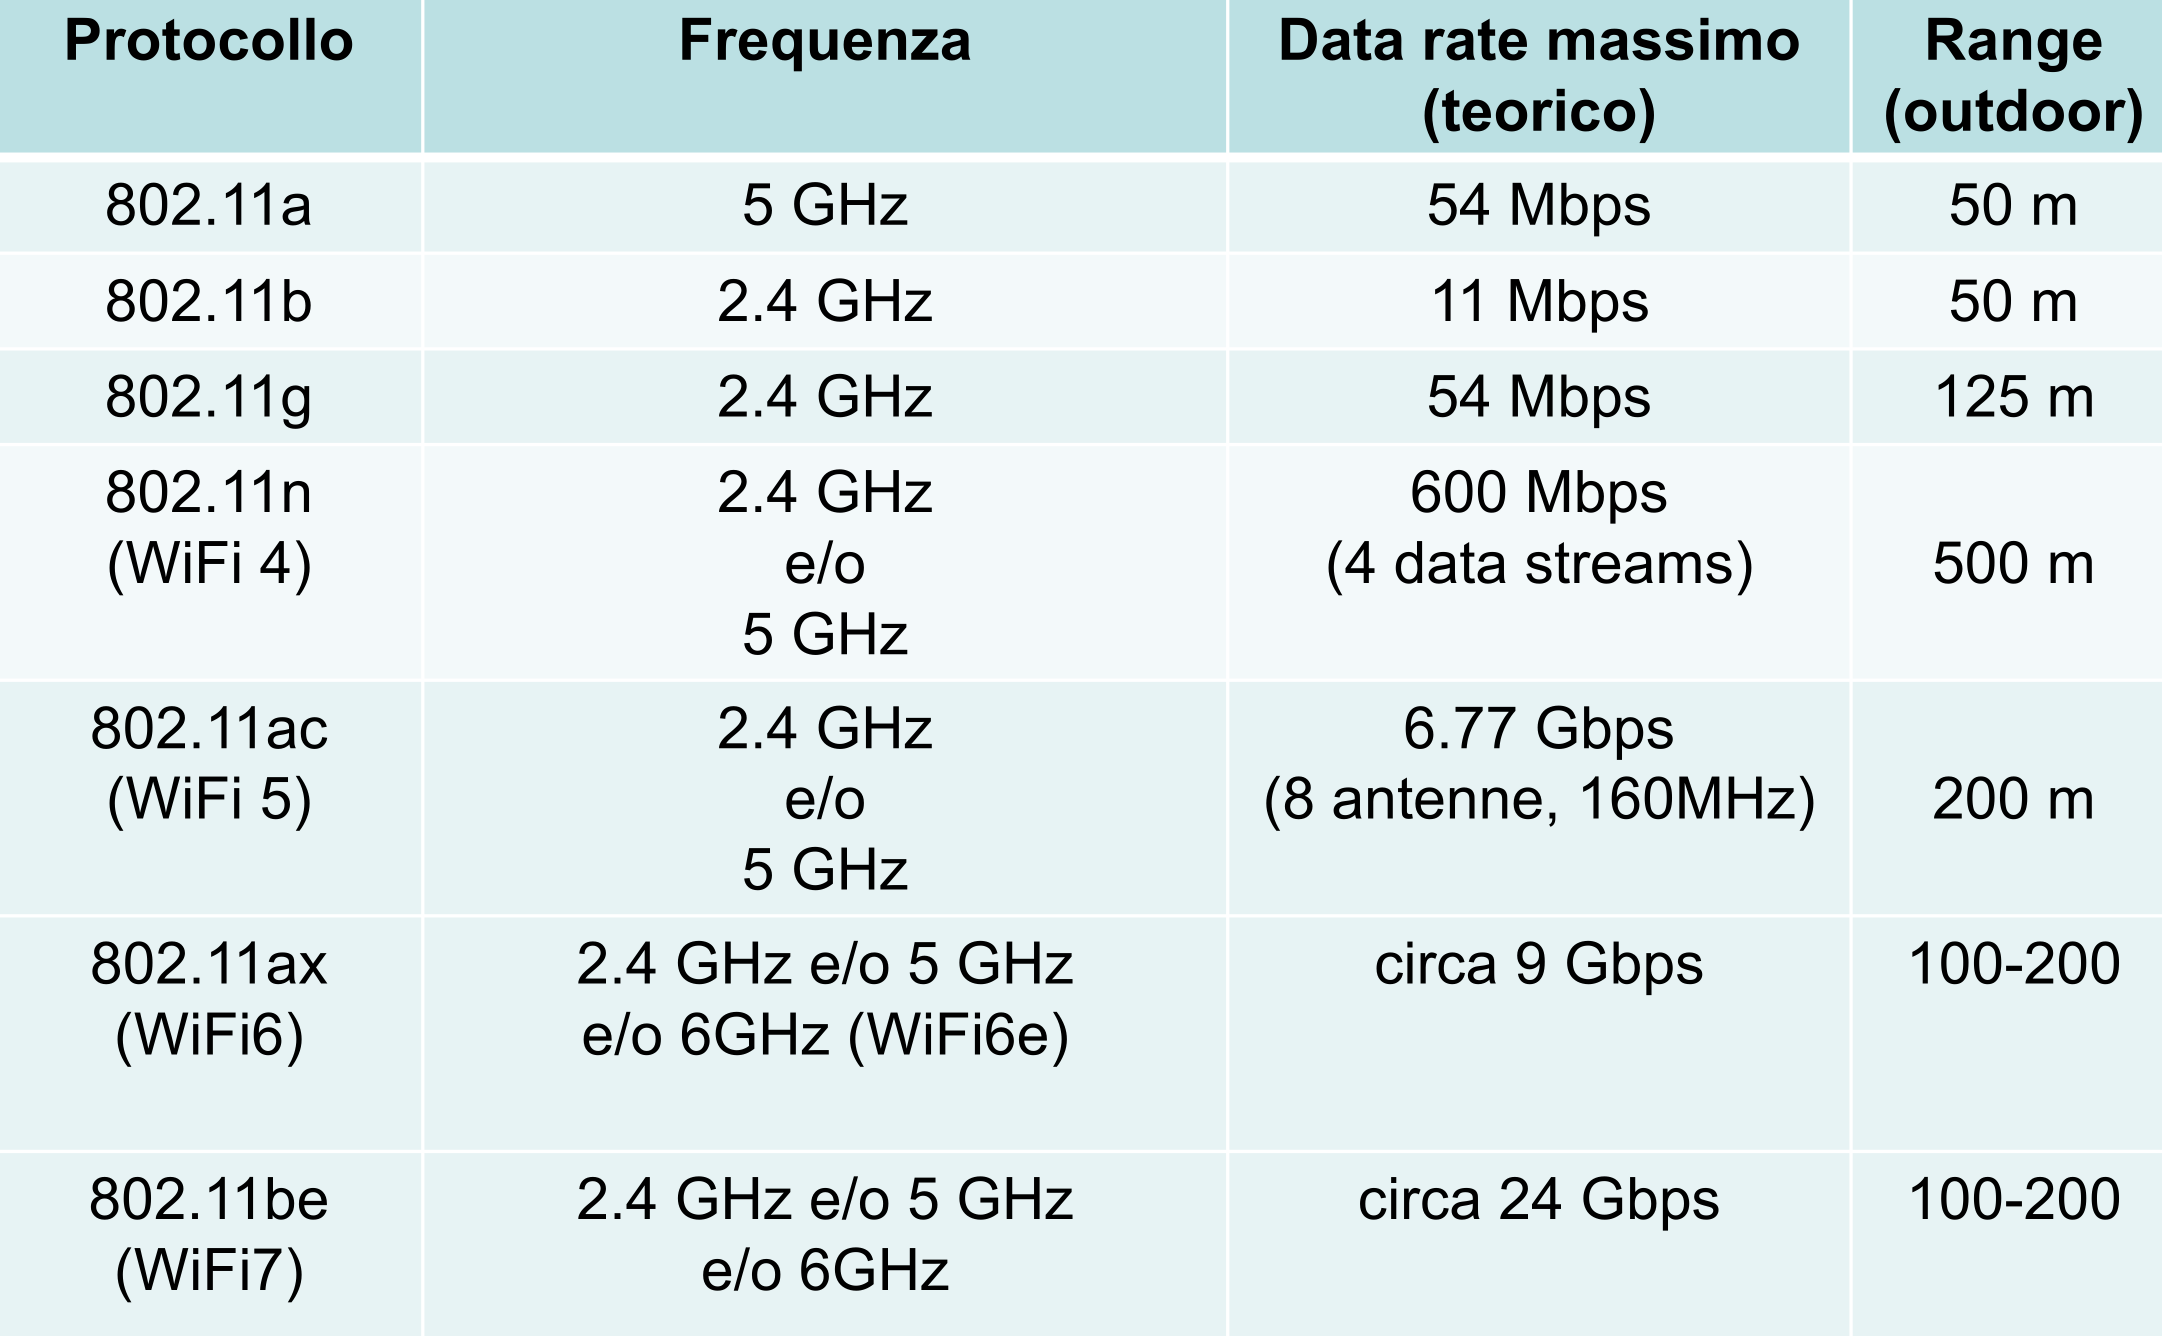
\includegraphics[width=\linewidth]{images/famigliaieee802.png}
        \caption{802.11x}
    \end{minipage}
\end{figure}

\subsection{Struttura dei canali 802.11b}
Nello standard 802.11b la banda radio viene suddivisa in 14 canali, le "onde" rappresentano l'ampiezza di banda di ogni canale wireless.

Seguendo queste ampiezze si possono invididuare le terne di canali che non interferiscono tra di loro, ad esempio 1, 6, 11; a conti fatti ogni canale ha dopo 5 canali quello con cui non interferisce.

Queste terne coprono l'area di interesse della rete wireless senza avere interferenze.
\begin{figure}[h!]
    \centering
    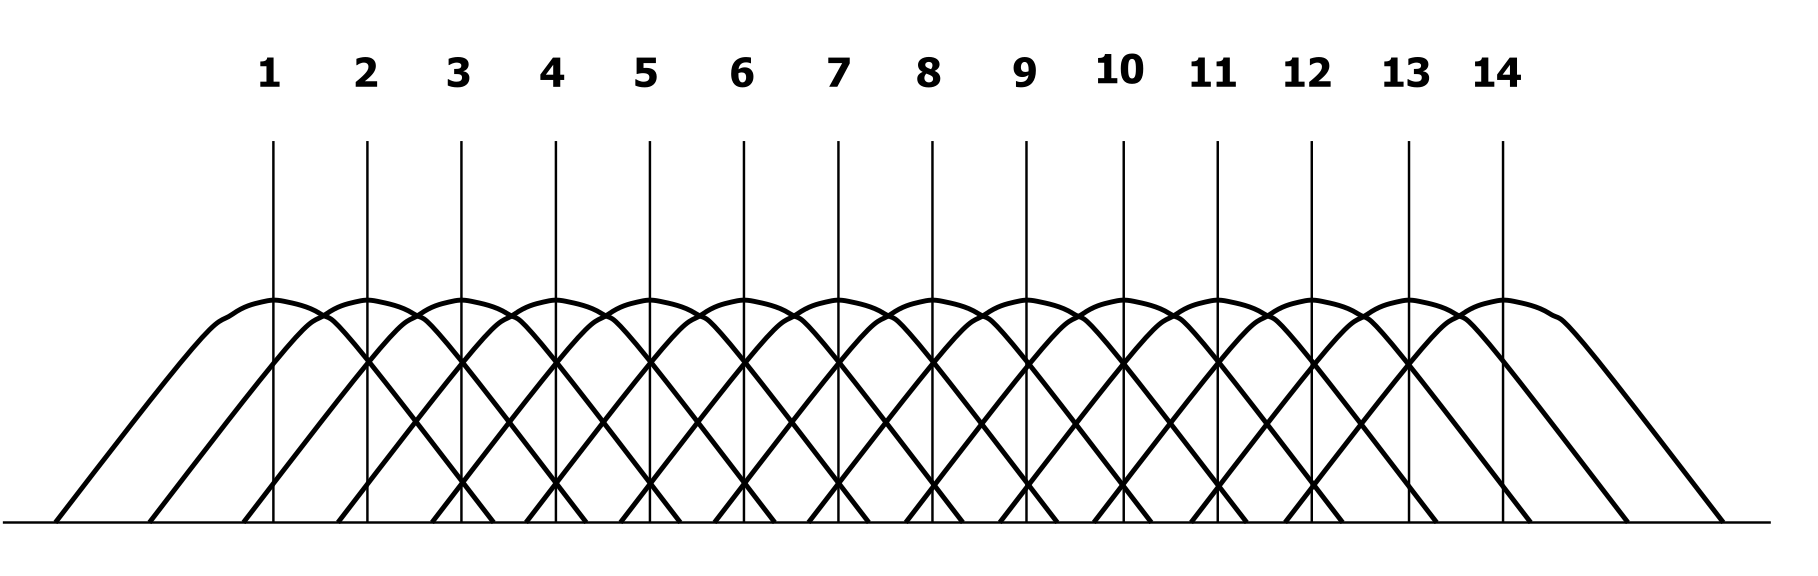
\includegraphics[scale=0.225]{images/canali802.png}
    \caption{Struttura canali 802.11b}
    \label{fig:strutturacanali}
\end{figure}




\begin{figure}[h!]
    \centering
    \begin{minipage}{0.35\textwidth}
        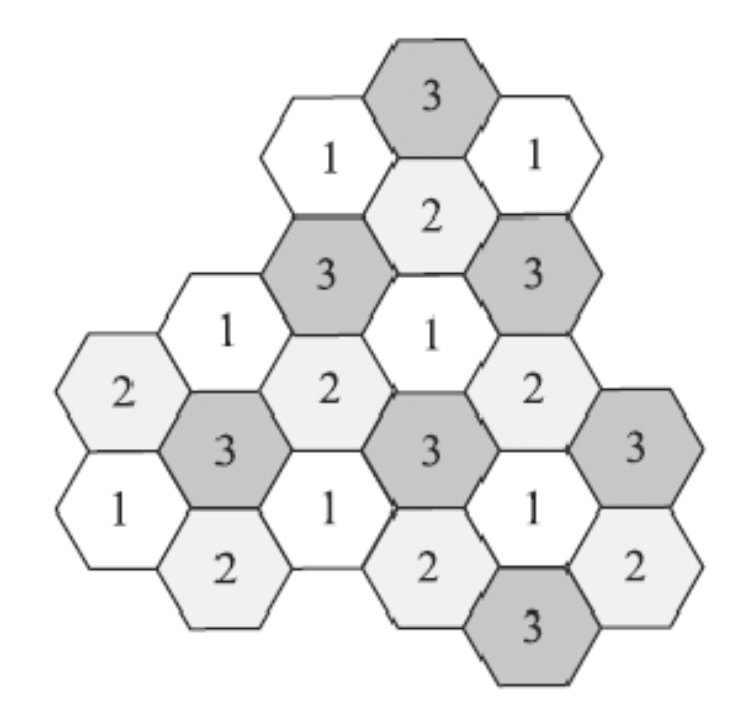
\includegraphics[width=\linewidth]{images/cluster3celle.png}
    \end{minipage}
    \hfill
    \begin{minipage}{0.5\textwidth}
        \paragraph{Cluster}
        In questa rappresentazione ogni esagono rappresenta una cella o area di copertura di un access point (AP). I numeri all'interno degli esagoni indicano il canale utilizzato da ciascun AP.
        
        Questa configurazione permette di minimizzare le interferenze tra le celle adiacenti, ottimizzando le prestazioni della rete wireless.
    \end{minipage}
    \caption{Cluster di 3 celle (1,2,3)}
    \label{fig:cluster3celle}
\end{figure}
\newpage
\subsubsection{Distributed Coordination Function (DCF)}
La WLAN usa il CSMA/CA, la DCF è insieme di regole per la gestione dell’accesso al
mezzo condiviso.

\begin{figure}[h!]
    \centering
    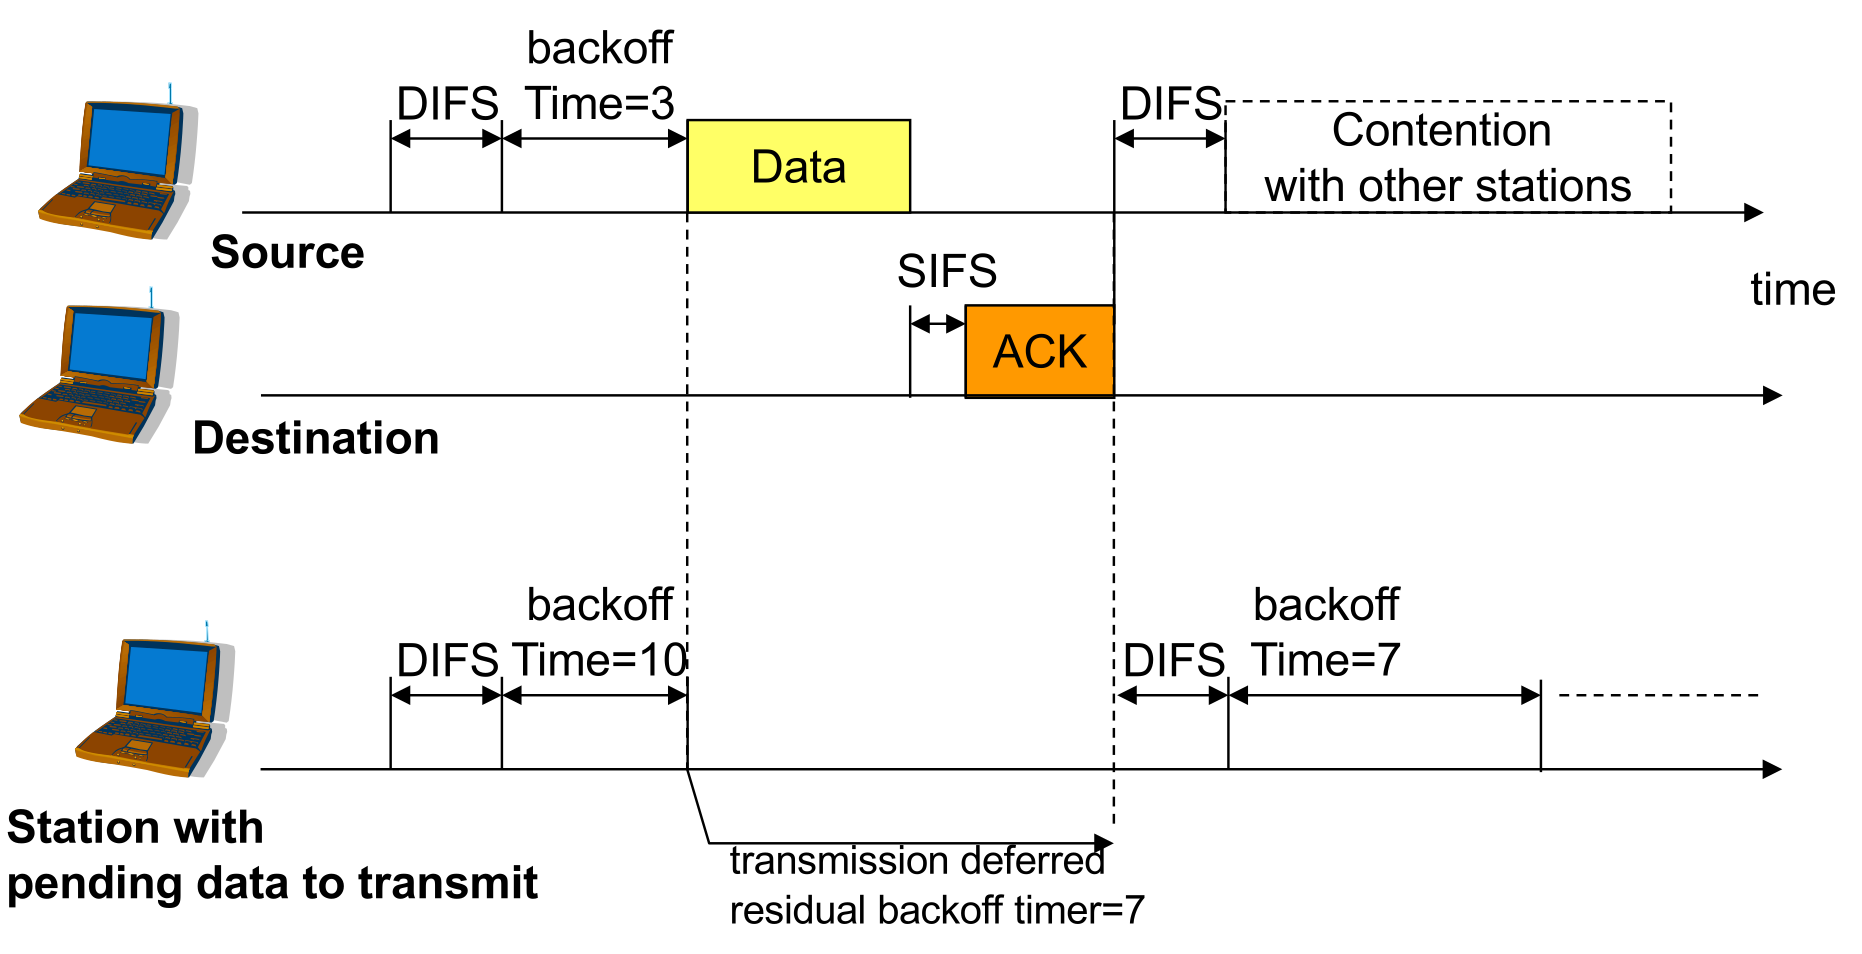
\includegraphics[scale=0.25]{images/dcf.png}
    \caption{Distributed Coordination Function (DCF)}
    \label{fig:dcf}
\end{figure}

Source ha interesse di comunicare qualcosa(data) a destination, per farlo utilizza la tecnologia WNAL e perciò non può inviare direttamente l'informazione al destinatario ma lo fa attraverso un'ulteriore stazione, un access point(station with pending data to transmit).

Source ascolta il canale per un certo periodo prima di far partire la comunicazione(CSMA/CA), precisamente aspetta un tempo DIFS + backoff, rispettivamente:
\begin{itemize}
    \item DIFS(DCF inter frame space): specifica la modalità di CSMA/CA utilizzata dal sistema, specifica per 802.11  
    \item backoff time: tempo calcolato tramite algoritmo di backoff, per decidere il tempo di subentro in trasmissione, source e la stazione hanno dei backoff time diversi in questo caso
\end{itemize}
Nel momento in cui source inizia ad inviare i dati, il backoff time della stazione si interrompe(proseguirrà solo al termine della comuniazione tra source e destination, poichè comunicano grazie alla station).

Source aspetta un riscontro(ACK) da parte di destination, che attenderà per un tempo SIFS(Short inter frame space), ossia un tempo predefinito che viene fornito al destination per assicurarsi di aver terminato correttamente i processi di ricezione, pronto per trasmettere l'ACK nel modo più corretto possibile. Una volta ricevuto l'ACK, la comunicazione è terminata.

Quello che si vede successivamente nell'immagine, la "Contention with other stations", indica una possibile contesa con altre "source" per l'utilizzo della stazione per la tramissione.

C'è sempre contesa tra gli apparati per poter comunicare con questa tecnologia. 

\newpage
\subsection{Nodi nascosti ed esposti}
Questi problemi esistono poichè i nodi condividono gli stessi canali per la condivisione.
\paragraph{Nodo nascosto}
I nodi “nascosti” (A e C) comunicano con B; i frame collidono nei pressi del nodo B.
\begin{figure}[h!]
    \centering
    \begin{minipage}{0.49\textwidth}
        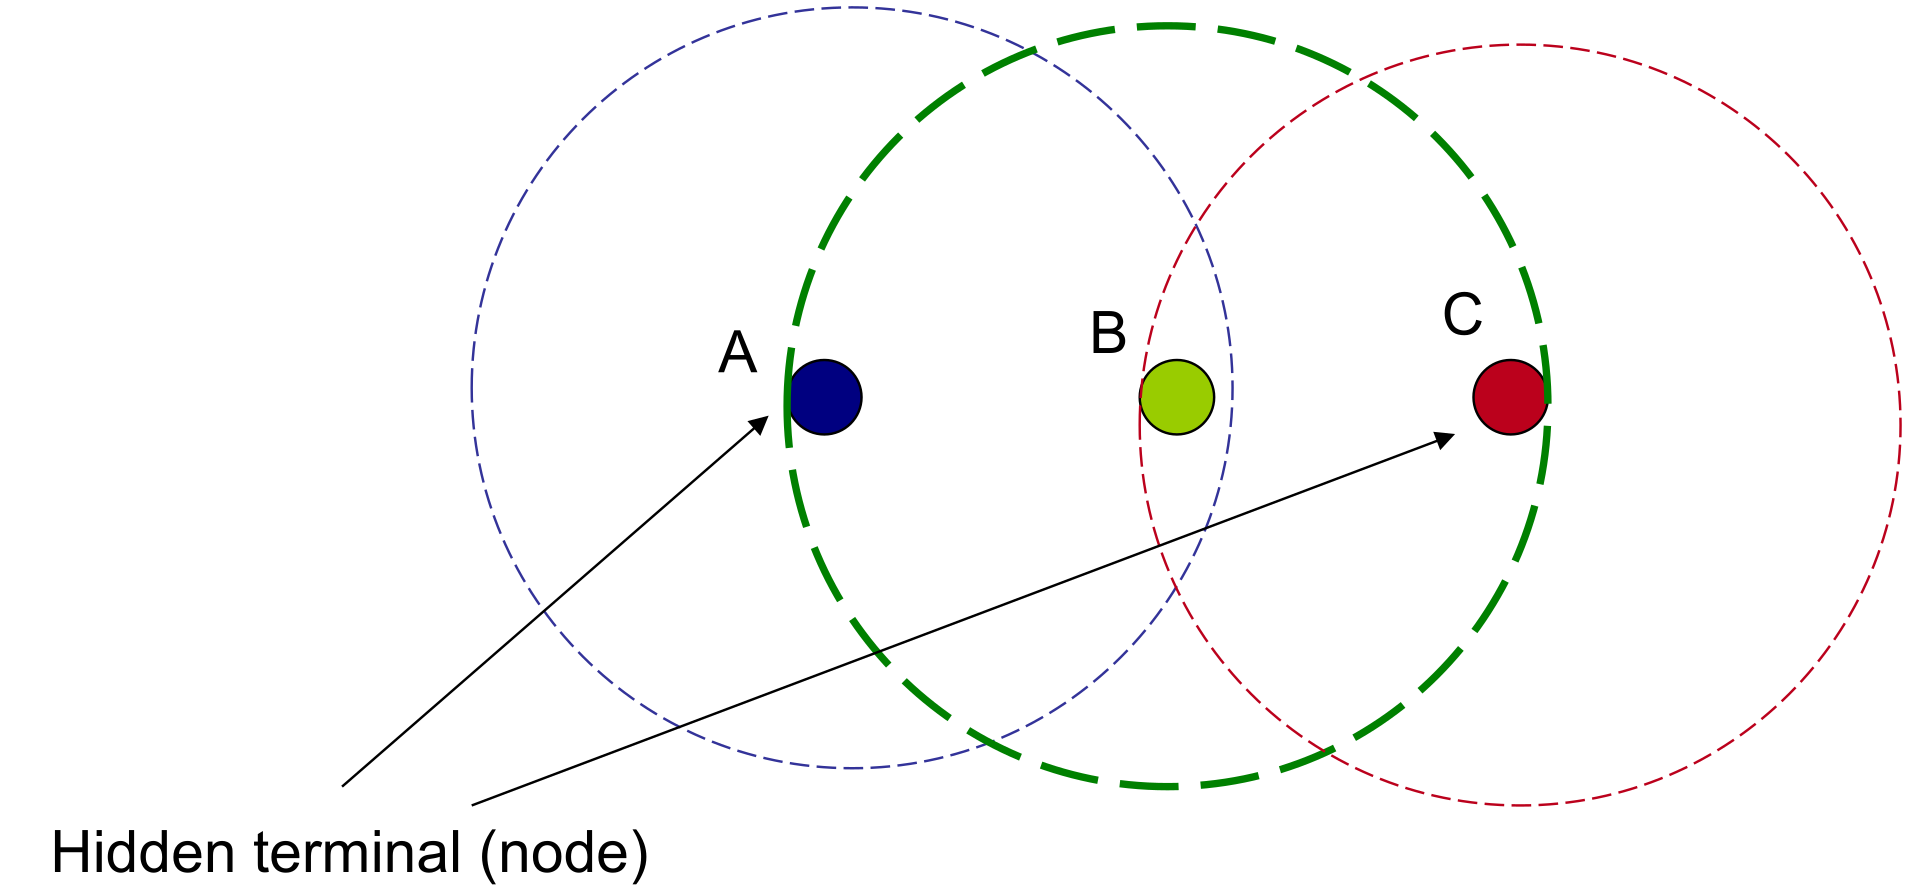
\includegraphics[width=\linewidth]{images/nodonascosto.png}
    \end{minipage}
    \hfill
    \begin{minipage}{0.5\textwidth}
        \paragraph{Nodo nascosto}
        Il nodo nascosto è un problema che si verifica nelle reti wireless quando due nodi non sono in grado di "vedersi" a vicenda a causa di ostacoli o distanza, ma entrambi possono comunicare con un terzo nodo. Ciò può portare a collisioni di pacchetti e perdita di dati.
    \end{minipage}
    \caption{Nodo nascosto}
    \label{fig:nodo nascosto}
\end{figure}

\subsubsection{Soluzione nodo nascosto} 

\begin{figure}[h!]
    \centering
    \begin{minipage}{0.5\textwidth}
\paragraph{Request to send RTS - 20 byte}
I nodi che intendono trasmettere tramite un nodo intermedio devono inviare un piccolo frame di richiesta, detto Request to send (RTS).

Inoltre la probabilità che ci sia una collisione, quindi un problema, con l'invio di questi pacchetti è molto bassa poichè sono molto piccoli.

\paragraph{Clear to send CTS - 14 byte}
Il nodo destinatario del frame RTS, conferma ed autorizza la richiesta inviando a sua volta un pacchetto piccolo, il Clear o send (CTS),  al nodo che ha inviato la richiesta.
    \end{minipage}
    \hfill
    \begin{minipage}{0.49\textwidth}
        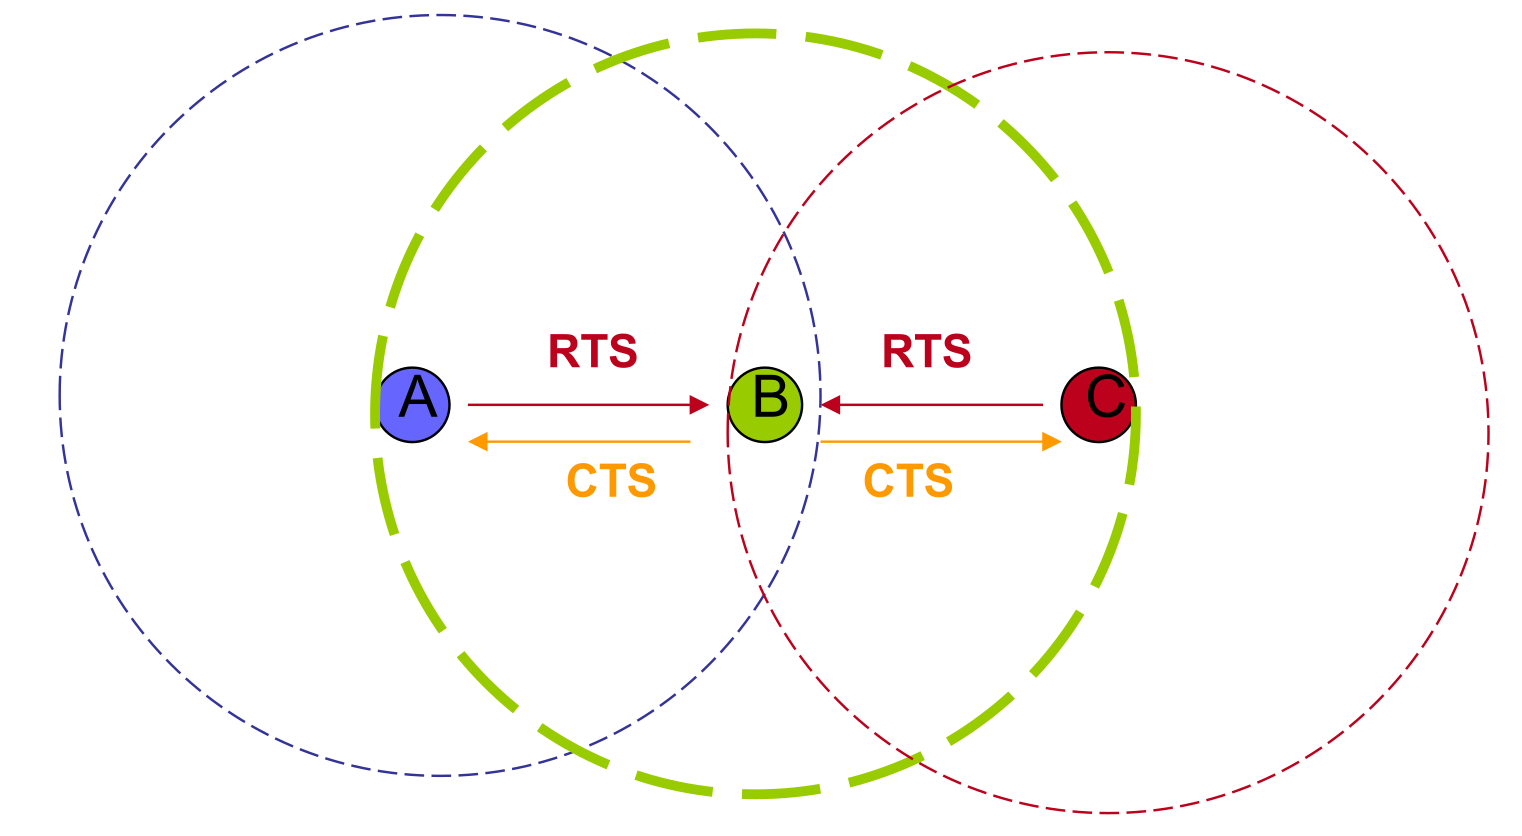
\includegraphics[width=\linewidth]{images/soluzionenodonascosto.png}
    \end{minipage}
    \caption{Soluzione nodo nascosto}
    \label{fig:soluzionenodonascosto}
\end{figure}

\begin{figure}[h!]
    \centering
    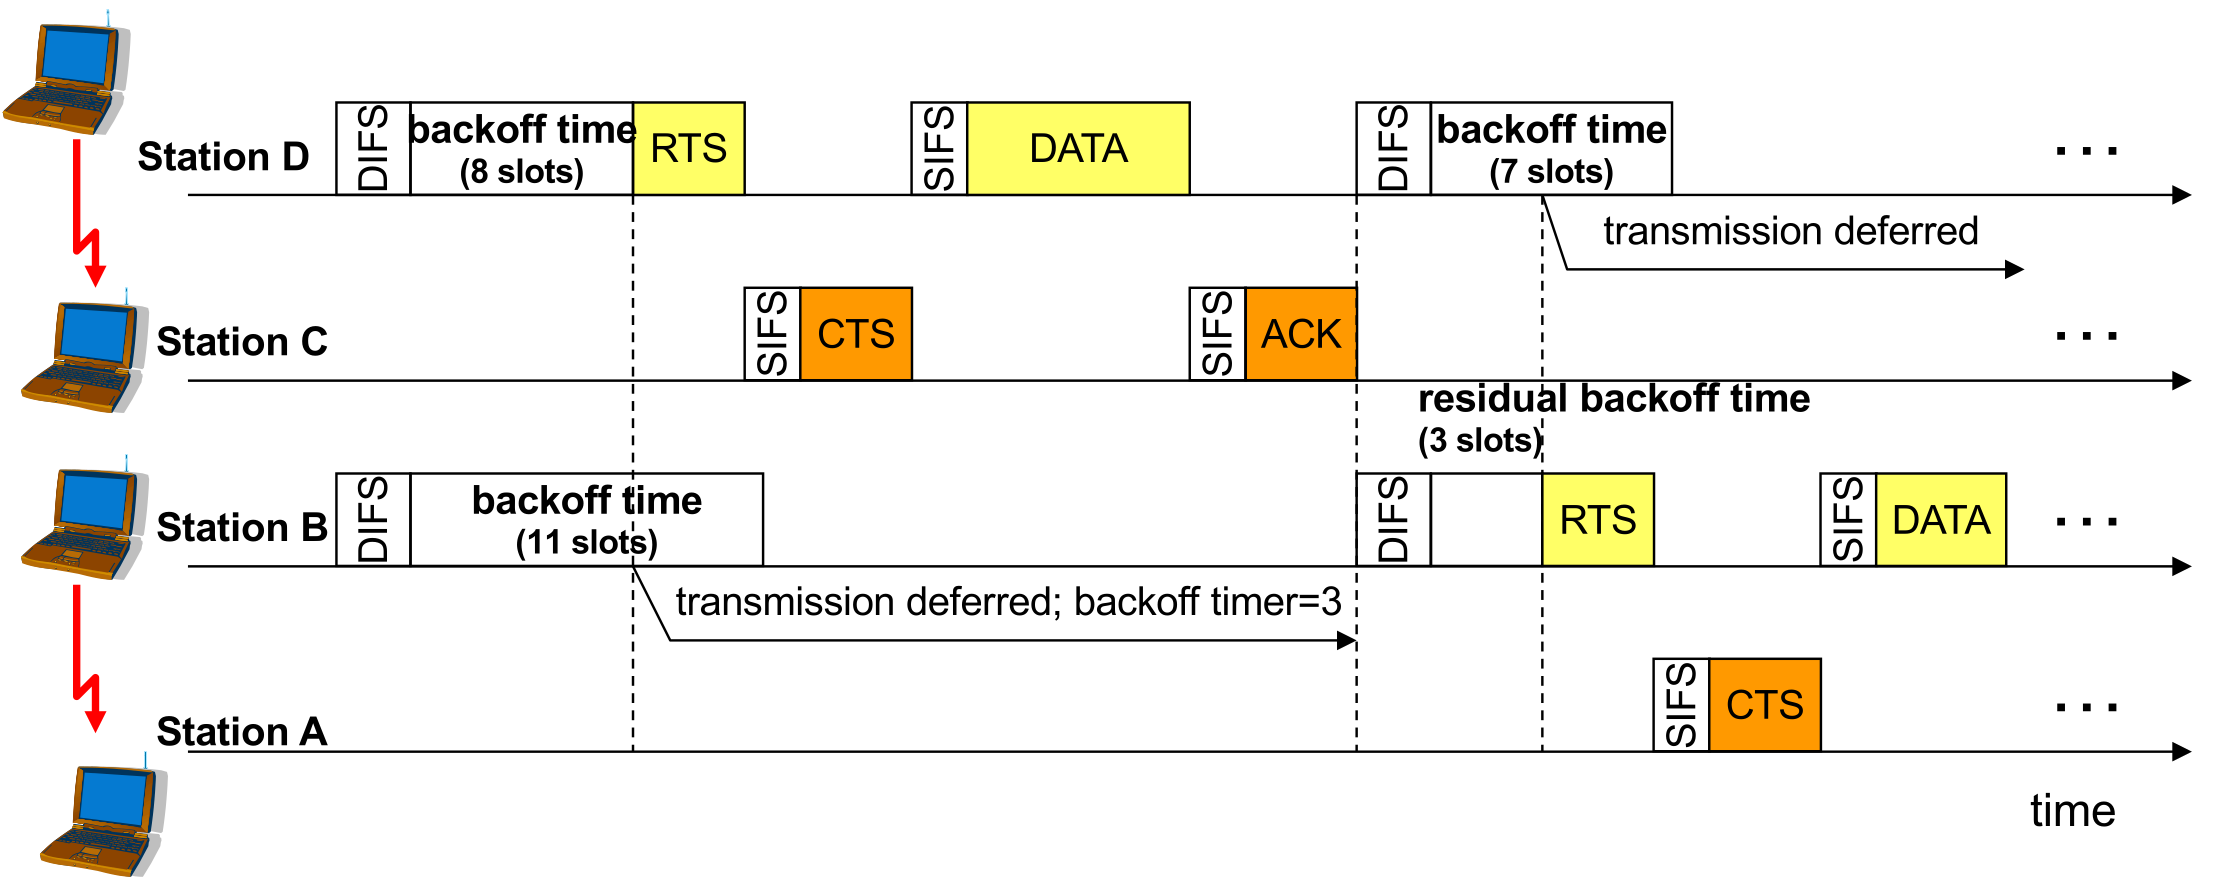
\includegraphics[scale=0.2]{images/dcfhandshake.png}
    \caption{Handshake DCF per nodi nascosti}
    \label{fig:dcfhandshake}
\end{figure}
Esempio della tramissione WLAN  802.11 con RTS e CTS. Di fatto cambia solo il tempo della duration, prima era composta da data, SIFS e ACK; adesso includo i campi RTS e CTS come in figura.


\newpage

\paragraph{Nodo esposto}

\begin{figure}[h!]
    \centering
    \begin{minipage}{0.49\textwidth}
        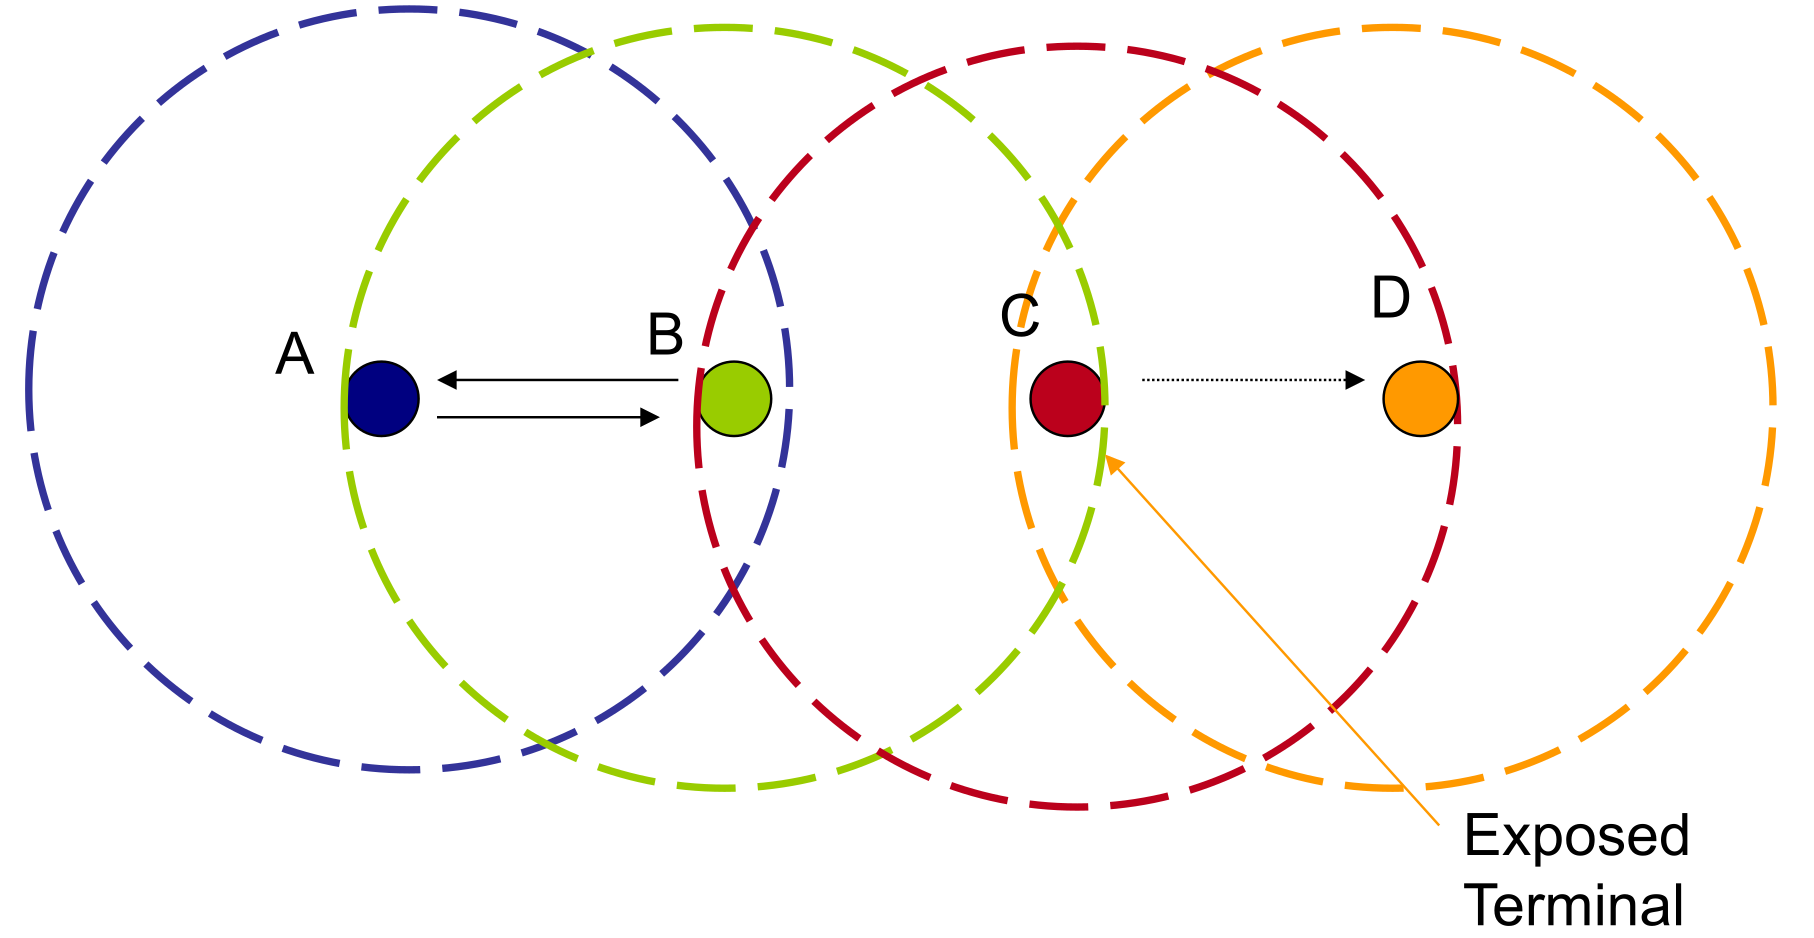
\includegraphics[width=\linewidth]{images/nodoesposto.png}
    \end{minipage}
    \hfill
    \begin{minipage}{0.5\textwidth}
        \paragraph{Nodo esposto}
        A e B stanno comunicando ed occupano il canale; il nodo C vuole comunicare con il canale D ma sente, tramite rilevazione di canale, che questo è già occupato.

        Questo si risolve avviando un backoff time(casuale, secondo un algoritmo) a fine comunicazione trasmessa con successo così che tra un pacchetto e l'altro, di quelli inviati da A e B, ci sia "spazio" per le comunicazioni di C e D, che rilevavano il canale occupato.
    \end{minipage}
    \caption{Nodo esposto}
    \label{fig:nodo esposto}
\end{figure}


\subsection{Dispositivi wireless}

\subsubsection{Hub}
L'hub è un dispositivo che riceve i dati da una stazione e li ritrasmette a tutte le altre stazioni collegate. In ambito wireless, l'hub non viene praticamente mai utilizzato perché non è in grado di gestire le collisioni e non offre alcuna forma di filtraggio o instradamento dei dati. In generale, l'hub lavora a livello fisico (livello 1 ISO/OSI).

\subsubsection{Bridge}
Il bridge è un dispositivo che collega due segmenti di rete, anche di tipo diverso (ad esempio una rete cablata e una wireless), filtrando il traffico in base agli indirizzi MAC. In ambito wireless, il bridge permette di collegare due reti wireless o una rete wireless e una cablata, inoltrando solo i frame destinati all'altro segmento. Opera a livello data link (livello 2 ISO/OSI).

\subsubsection{Switch}
Lo switch è un dispositivo che riceve i frame e li inoltra solo alla porta (o interfaccia) corretta, in base all'indirizzo MAC di destinazione. In ambito wireless, la funzione di switch è spesso integrata negli access point avanzati, che possono gestire più connessioni e segmentare il traffico tra i dispositivi collegati. Anche lo switch opera a livello data link (livello 2 ISO/OSI).
\subsubsection{Modalità di funzionamento di uno switch}

\begin{itemize}
    \item \textbf{Store and Forward}:\\
    Lo switch legge l’intero frame e verifica il campo FCS (scarta il frame se errato). Il frame viene memorizzato temporaneamente nel buffer associato alla porta d’uscita e trasmesso quando la linea della porta d’uscita è libera.
    \item \textbf{Cut and Through}:\\
    Lo switch legge solo l’header del frame e inoltra immediatamente il frame senza memorizzazione intermedia. Il ritardo di elaborazione è indipendente dalla dimensione del frame.
    \item \textbf{Fragment Free}:\\
    Lo switch legge solo i primi 64 byte del frame (dimensione minima frame Ethernet) per evitare di inoltrare frame che potrebbero essere coinvolti in collisioni. I frame di dimensione minore a 64 byte vengono scartati.
\end{itemize}
CAPIRE SE FINIRE FILE 11